\documentclass[a4paper,11pt]{article}
\usepackage[utf8]{inputenc}
%

\usepackage[utf8]{inputenc}%Packages
\usepackage[T1]{fontenc}
\usepackage{fourier} 
\usepackage[english]{babel} 
\usepackage{amsmath,amsfonts,amsthm} 
\usepackage{lscape}
\usepackage{geometry}
\usepackage{amsmath}
\usepackage{algorithm}
\usepackage{algorithmic}
\usepackage{amssymb}
\usepackage{amsfonts}
\usepackage{times}
\usepackage{bm}
\usepackage{mathtools}
\usepackage{ stmaryrd }
\usepackage{ amssymb }
\usepackage{ textcomp }
\usepackage[normalem]{ulem}
% For derivation rules
\usepackage{mathpartir}
\usepackage{color}
\usepackage{a4wide}

\usepackage{stmaryrd}
\SetSymbolFont{stmry}{bold}{U}{stmry}{m}{n}

\newcommand{\distr}{\mathsf{Distr}}
\newcommand{\uniform}{\mathsf{unif}}
\newcommand{\pdf}{\mathsf{pdf}}
\newcommand{\snap}{\mathsf{Snap}}
\newcommand{\fsnap}{\mathsf{Snap}_{\mathbb{F}}}
\newcommand{\rsnap}{\mathsf{Snap}_{\mathbb{R}}}


\newcommand{\pr}[2]{\underset{#1}{\mathsf{Pr}}[#2]}
\newcommand{\projl}{\pi_1}
\newcommand{\projr}{\pi_2}
\newcommand{\supp}{\mathsf{supp}}
\newcommand{\clamp}{\mathsf{clamp}}
\newcommand{\real}{\mathbb{R}}
\newcommand{\samplel}{\xleftarrow{\$}}
\newcommand{\psup}{\mathsf{Sup}}
\newcommand{\sign}{\mathsf{sign}}

\newcommand{\lapmech}{\mathcal{L}}
\newcommand{\laplace}{\mathsf{laplce}}
\newcommand{\round}[1]{\lfloor #1 \rceil}


%for syntax:

%for programs:
\newcommand{\prog}{p}
\newcommand{\fprog}{p_{\mathbb{F}}}
\newcommand{\rprog}{p_{\mathbb{R}}}
\newcommand{\ret}{\mathsf{return}}



%expression
\newcommand{\expr}{e}
\newcommand{\fexpr}{\expr_{\mathbb{F}}}
\newcommand{\rexpr}{\expr_{\mathbb{R}}}

\newcommand{\elet}{\kw{let}}

\newcommand{\ein}{\kw{in}}

%for smaples:
\newcommand{\bernoulli}{\kw{bernoulli}}

%values
\newcommand{\fval}{c}
\newcommand{\rval}{r}
\newcommand{\valv}{v}
\newcommand{\data}{D}

%variables
\newcommand{\varx}{x}

\newcommand{\fvarx}{x}
\newcommand{\rvarx}{X}


\newcommand{\term}{t}
\newcommand{\etrue}{\kw{true}}
\newcommand{\efalse}{\kw{false}}
% \newcommand{\eflconst}{c}
% \newcommand{\erlconst}{r}
\newcommand{\precision}{\eta}
\newcommand{\floaten}{\kw{fl}}

\newcommand{\err}{err}
\newcommand{\condition}{\Phi}
\newcommand{\edistr}{\mu}

\newcommand{\fbigstep}{\Downarrow^{\mathbb{F}}}
\newcommand{\rbigstep}{\Downarrow^{\mathbb{R}}}

\newcommand{\bigstep}{\Downarrow}
\newcommand{\trsto}{\Rightarrow}


%for environments
\newcommand{\trsenv}{\Theta}

\newcommand{\evlenv}{\Gamma}

\newcommand{\fevlenv}{\Gamma^{\mathbb{F}}}

\newcommand{\revlenv}{\Gamma^{\mathbb{R}}}



\usepackage{stackengine} 

% For Operations
%binary operations
\newcommand{\bop}{*}
\newcommand{\obop}{\stackMath\mathbin{\stackinset{c}{0ex}{c}{0ex}{\text{\footnotesize{$\bop$}}}{\bigcirc}}}

\newcommand{\oexp}{\stackMath\mathbin{\stackinset{c}{0ex}{c}{0ex}{\text{\footnotesize{$\mathsf{e}$}}}{\bigcirc}}}

\newcommand{\oln}{\stackMath\mathbin{\stackinset{c}{0ex}{c}{0ex}{\text{\footnotesize{$\mathsf{ln}$}}}{\bigcirc}}}

\newcommand{\odiv}{\stackMath\mathbin{\stackinset{c}{0ex}{c}{0ex}{\text{\footnotesize{$\div$}}}{\bigcirc}}}
\newcommand{\ubar}[1]{\text{\b{$#1$}}}

%unary operations
\newcommand{\uop}{\circ}
\newcommand{\ouop}{\stackMath\mathbin{\stackinset{c}{0ex}{c}{0ex}{\text{\footnotesize{$\uop$}}}{\bigcirc}}}





\newcommand{\diam}{{\color{red}\diamond}}
\newcommand{\dagg}{{\color{blue}\dagger}}
\let\oldstar\star
\renewcommand{\star}{\oldstar}

\newcommand{\im}[1]{\ensuremath{#1}}

\newcommand{\kw}[1]{\im{\mathtt{#1}}}


\newcommand{\set}[1]{\im{\{{#1}\}}}

\newcommand{\mmax}{\ensuremath{\mathsf{max}}}

%%%%%%%%%%%%%%%%%%%%%%%%%%%%%%%%%%%%%%%%%%%%%%%%%%%%%%%%
% Comments
\newcommand{\omitthis}[1]{}

% Misc.
\newcommand{\etal}{\textit{et al.}}
\newcommand{\bump}{\hspace{3.5pt}}

% Text fonts
\newcommand{\tbf}[1]{\textbf{#1}}
%\newcommand{\trm}[1]{\textrm{#1}}

% Math fonts
\newcommand{\mbb}[1]{\mathbb{#1}}
\newcommand{\mbf}[1]{\mathbf{#1}}
\newcommand{\mrm}[1]{\mathrm{#1}}
\newcommand{\mtt}[1]{\mathtt{#1}}
\newcommand{\mcal}[1]{\mathcal{#1}}
\newcommand{\mfrak}[1]{\mathfrak{#1}}
\newcommand{\msf}[1]{\mathsf{#1}}
\newcommand{\mscr}[1]{\mathscr{#1}}

% Text mode
\newenvironment{nop}{}{}

% Math mode
\newenvironment{sdisplaymath}{
\begin{nop}\small\begin{displaymath}}{
\end{displaymath}\end{nop}\ignorespacesafterend}
\newenvironment{fdisplaymath}{
\begin{nop}\footnotesize\begin{displaymath}}{
\end{displaymath}\end{nop}\ignorespacesafterend}
\newenvironment{smathpar}{
\begin{nop}\small\begin{mathpar}}{
\end{mathpar}\end{nop}\ignorespacesafterend}
\newenvironment{fmathpar}{
\begin{nop}\footnotesize\begin{mathpar}}{
\end{mathpar}\end{nop}\ignorespacesafterend}
\newenvironment{alignS}{
\begin{nop}\begin{align}}{
\end{align}\end{nop}\ignorespacesafterend}
\newenvironment{salignS}{
\begin{nop}\small\begin{align}}{
\end{align}\end{nop}\ignorespacesafterend}
\newenvironment{falignS}{
\begin{nop}\footnotesize\begin{align*}}{
\end{align}\end{nop}\ignorespacesafterend}

% Stack formatting
\newenvironment{stackAux}[2]{%
\setlength{\arraycolsep}{0pt}
\begin{array}[#1]{#2}}{
\end{array}}
\newenvironment{stackCC}{
\begin{stackAux}{c}{c}}{\end{stackAux}}
\newenvironment{stackCL}{
\begin{stackAux}{c}{l}}{\end{stackAux}}
\newenvironment{stackTL}{
\begin{stackAux}{t}{l}}{\end{stackAux}}
\newenvironment{stackTR}{
\begin{stackAux}{t}{r}}{\end{stackAux}}
\newenvironment{stackBC}{
\begin{stackAux}{b}{c}}{\end{stackAux}}
\newenvironment{stackBL}{
\begin{stackAux}{b}{l}}{\end{stackAux}}

%APPENDIX
\newcommand{\caseL}[1]{\item[\textbf{case}] \textbf{#1}\newline}
\newcommand{\subcaseL}[1]{\item[\textbf{subcase}] \textbf{#1}\newline}

\newcommand{\todo}[1]{{\footnotesize \color{red}\textbf{[[ #1 ]]}}}


%% \makeatletter
%% \newcommand\definitionname{Lemma}
%% \newcommand\listdefinitionname{Proofs of Lemmas and Theorems}
%% \newcommand\listofdefinitions{%
%%   \section*{\listdefinitionname}\@starttoc{def}}
%% \makeatother



\newtheoremstyle{athm}{\topsep}{\topsep}%
      {\upshape}%         Body font
      {}%         Indent amount (empty = no indent, \parindent = para indent)
      {\bfseries}% Thm head font
      {}%        Punctuation after thm head
      {.8em}%     Space after thm head (\newline = linebreak)
      {\thmname{#1}\thmnumber{ #2}\thmnote{~\,(#3)}
% \addcontentsline{Lemma}{Lemma}
%   {\protect\numberline{\thechapter.\thelemma}#1}
      % \ifstrempty{#3}%
      {\addcontentsline{def}{section}{#1~#2~#3}}%
      % {\addcontentsline{def}{subsection}{\theathm~#3}}
\newline}%         Thm head spec

 \theoremstyle{athm}


% \newtheoremstyle{break}
%   {\topsep}{\topsep}%
%   {\itshape}{}%
%   {\bfseries}{}%
%   {\newline}{}%
% \theoremstyle{break}

%There are some problems with llncs documentcalss, so commenting these out until i find a solution
\newtheorem{thm}{Theorem}

%\spnewtheorem{thm1}[theorem]{Theorem}{\bfseries}{\upshape}
%\newenvironment{Theorem}[1][]{\begin{thm1}\iffirstargument[#1]\fi\quad\\}{\end{thm1}}

 \newtheorem{lem}[thm]{Lemma}
 \newtheorem{conjec}{Conjecture}
 \newtheorem{corr}[thm]{Corollary}
 \newtheorem{defn}{Definition}
 \newtheorem{prop}[thm]{Proposition}
 \newtheorem{assm}[thm]{Assumption}

\newtheorem{Eg}[thm]{Example}
\newtheorem{hypothesis}[thm]{Hypothesis}
\newtheorem{motivation}{Motivation}

% BNF symbols
\newcommand{\bnfalt}{{\bf \,\,\mid\,\,}}
\newcommand{\bnfdef}{{\bf ::=~}}

%% Highlighting
\newcommand{\hlm}[1]{\mbox{\hl{$#1$}}}

%% Provenance modes
\newcommand{\modifrcationProvenance}{{\bf MP}}
\newcommand{\updateProvenance}{{\bf UP}}

%Lemmas
\newcommand{\lemref}[1]{Lemma \ref{#1}} %name and number
\newcommand{\thmref}[1]{Theorem \ref{#1}} %name and number

\renewcommand{\labelenumii}{\theenumii}
\renewcommand{\theenumii}{\theenumi.\arabic{enumii}.}

\usepackage{enumitem}
\setenumerate{listparindent=\parindent}

\newlist{enumih}{enumerate}{3}
\setlist[enumih]{label=\alph*),before=\raggedright, topsep=1ex, parsep=0pt,  itemsep=1pt }

\newlist{enumconc}{enumerate}{3}
\setlist[enumconc]{leftmargin=0.5cm, label*= \arabic*.  , topsep=1ex, parsep=0pt,  itemsep=3pt }

\newlist{enumsub}{enumerate}{3}
\setlist[enumsub]{ leftmargin=0.7cm, label*= \textbf{subcase} \bf \arabic*: }

\newlist{enumsubsub}{enumerate}{3}
\setlist[enumsubsub]{ leftmargin=0.5cm, label*= \textbf{subsubcase} \bf \arabic*: }

\newlist{mainitem}{itemize}{3}
\setlist[mainitem]{ leftmargin=0cm , label= {\bf Case} }


\newenvironment{subproof}[1][\proofname]{%
  \renewcommand{\qedsymbol}{$\blacksquare$}%
  \begin{proof}[#1]%
}{%
  \end{proof}%
}


\newenvironment{nstabbing}
  {\setlength{\topsep}{0pt}%
   \setlength{\partopsep}{0pt}%
   \tabbing}
  {\endtabbing} 





%%% Local Variables:
%%% mode: latex
%%% TeX-master: "main"
%%% End:

\usepackage{eucal}
\usepackage{url}
\usepackage{tikz}
\begin{document}

\title{Verifying Snapping Mechanism}

\maketitle
In order to verify the differential privacy proeprty of the snapping mechanism\cite{mironov2012significance}, we follow the logic rules designed from \cite{barthe2016proving}.

Some new rules are added into this logic in Figure \ref{logic_rule} following with correctness proof. Then we formalized the snapping mechanism and verified its differential privacy property under these logic rules.

\section{Program Logic}
\begin{defn}
[Laplce mechanism \cite{dwork2006calibrating}]
Let $\epsilon > 0$. The Laplace mechanism  $\lapmech_{\epsilon}$: $\real \to \distr(\real)$ is defined by $\lapmech(t) = t + v$, where $v \in \real$ is drawn from the Laplace distri bution $\laplace(\frac{1}{\epsilon})$.
\end{defn}

\begin{defn}
Let $\epsilon \leq 0$. The $\epsilon${\text -DP divergence} $\Delta_{\epsilon}(\mu_1, \mu_2)$ between two sub-distributions $\mu_1 \in \distr(U)$, $\mu_2 \in \distr(U)$ is defined as:
\[	
	\underset{E \in U}{sup}\Big(\pr{x \leftarrow \mu_1}{x \in E} - \exp(\epsilon) \pr{x \leftarrow \mu_2}{x \in  E}]\Big)
\]

\end{defn}

\begin{defn}
[$(\epsilon, \delta)$ - lifting \cite{barthe2016proving}]
Two sub-distributions $\mu_1 \in \distr(U_1)$, $\mu_2 \in \distr(U_2)$are related by the $(\epsilon, \delta)$ - dilation lifting of $\Psi \subseteq U_1 \times U_2$, written $\mu_1 \Psi^{\#(\epsilon, \delta)} \mu_2$, if there exist two witness sub-distributions $\mu_L \in \distr(U_1 \times U_2)$ and $\mu_R \in \distr(U_1, U_2)$ s.t.:
\begin{enumerate}
	\item $\projl(\mu_L) = \mu_1$ and $\projr(\mu_R) = \mu_2$;
	\item $\supp(\mu_L) \subseteq \Psi$ and $\supp(\mu_R) \subseteq \Psi$; and
	\item $\Delta_{\epsilon}(\mu_L, \mu_R) \leq \delta$.
\end{enumerate}
\end{defn}

The logic rules we are using in our work is presented in Figure \ref{logic_rule}. The correctness of rules is proved in Theorem \ref{corr_axunif} and Theorem \ref{corr_axnull}

\begin{figure}
\begin{mathpar}
\inferrule*[right = AxUnif]
{
}
{
	\vdash 
	u_1 \samplel \mu 
	\sim_{\epsilon, 0} 
	u_2 \samplel \mu 
	: \top \Rightarrow  e^{-\epsilon} u_2 \leq u_1 \leq e^{\epsilon} u_2
}
\and
\inferrule*[right = LapGen]
{
}
{
	\vdash 
	y_1 \samplel \lapmech_{\epsilon}(e_1) 
	\sim_{k' \cdot \epsilon, 0} 
	y_2 \samplel \lapmech_{\epsilon}(e_2)
	: | k + e_1 - e_2| \leq k'  \Rightarrow  y_1 + k = y_2
}
\and
\inferrule*[right = LapNull]
{
}
{
	\vdash 
	y_1 \samplel \lapmech_{\epsilon}(e_1) 
	\sim_{0, 0} 
	y_2 \samplel \lapmech_{\epsilon}(e_2)
	: \top  \Rightarrow  y_1 - y_2 = e_1 - e_2
}
\and
\inferrule*[right = AxNull]
{
}
{
	\vdash 
	y_1 \samplel  \mu
	\sim_{0, 0} 
	y_2 \samplel \mu
	: \top  \Rightarrow  y_1 = y_2
}
\and
\inferrule*[right = Comp]
{
p_1 \sim_{k, 0} p_2 : \Phi_1 \Rightarrow \Phi'_1
\\
c_1 \sim_{k', 0} c_2 : \Phi'_1 \Rightarrow \Phi_2
}
{
	\vdash 
	p_1; c_1  
	\sim_{k + k', 0} 
	p_2; c_2
	: \Phi_1  \Rightarrow  \Phi_2
}
\end{mathpar}
\caption{Logic Rules from \cite{barthe2016proving}}
\label{logic_rule}
\end{figure}


\begin{thm}
\label{corr_axunif}
Let $\mu_1 \in \distr(\real)$, $\mu_2 \in \distr(\real)$ are defined:
\[
	{\mu_1}(x) = \uniform(x)
\]
\[
	{\mu_2}(y) = {\uniform}(y)
\]
where $\uniform$ is uniform distribution over $[0, 1)$ whoes $\pdf.$ is defined as:
\[
	\pdf_{\uniform}(x) = 
	\begin{cases}
	1 & x \in [0, 1)\\
	0       & o.w.
	\end{cases}.
\]
Then, $\mu_1 \Psi^{\#(\epsilon, 0)} \mu_2$, where
\[
	\Psi = \{(x,y) \in \real \times \real | x \cdot e^{-\epsilon} \leq y \leq x \cdot e^{\epsilon} \}
\]
\end{thm}

\begin{thm}
\label{corr_axnull}
For any distributions $\mu_1 \in \distr(\real)$, $\mu_2 \in \distr(\real)$, $\mu_1 \Psi^{\#(0, 0)} \mu_2$, where
\[
	\Psi = \{(x,y) \in \real \times \real | x = y \}
\]
\end{thm}


\begin{proof}[Proof of Theorem \ref{corr_axunif}]

Existing $\mu_L, \mu_R \in \distr(\real \times \real)$:
\[
	{\mu_L}(x, y) = 
	\begin{cases}
	{\uniform}(x) & x \cdot e^{-\epsilon} = y \land x \in [0, 1)\\
	0       & o.w.
	\end{cases}
	\\
	{\mu_R}(x, y) = 
	\begin{cases}
	{\uniform}(y) & x \cdot e^{-\epsilon} = y \land y \in [0, 1)\\
	0       & o.w.
	\end{cases}.
\]


Their $\pdf.$ are defined:
\[
	\pdf_{\mu_L}(x, y) = 
	\begin{cases}
	\pdf_{\uniform}(x) & x \cdot e^{-\epsilon} = y \land x \in [0, 1)\\
	0       & o.w.
	\end{cases}
\]
\[
	\pdf_{\mu_R}(x, y) = 
	\begin{cases}
	\pdf_{\uniform}(y) & x \cdot e^{-\epsilon} = y \land y \in [0, 1)\\
	0       & o.w.
	\end{cases}.
\]
\begin{itemize}
	\item $\supp(\mu_L) \in \Psi \land \supp(\mu_R) \in \Psi$

	\begin{itemize}
		\item $\supp(\mu_L) \subseteq \Psi$ 

		By definition of the $\pdf$ of $\mu_L$, we have: $\pr{(x,y) \samplel \mu_L}{(x,y) \notin \Psi} = 0$.

		Then we can derive $\supp(\mu_L) \in \Psi$

		\item $\supp(\mu_R) \subseteq \Psi$

		By definition of the $\pdf$ of $\mu_R$, we have: $\pr{(x,y) \samplel \mu_R}{(x,y) \notin \Psi} = 0$.

		Then we can derive $\supp(\mu_L) \in \Psi$

	\end{itemize}		


	\item $\projl(\mu_L) = \mu_1 \land \pi_2(\mu_R) = \mu_2$
	
	\begin{itemize}
		\item $\projl(\mu_L) = \mu_1$ 

		% Equivalent to show $\pdf_{\projl(\mu_L)}  = \pdf_{\mu_1}$.

		By definition of the $\projl$ and $\pdf$ of $\mu_L$, we have $\forall x \in \real$:
		\[
			\pdf_{\projl(\mu_L)}(x) = 
			\begin{cases}
			\int_{y}\pdf_{\uniform}(x) & (x,y) \in \Psi \land x \in [0, 1)\\
			0       & o.w.
			\end{cases} 
			= 
			\begin{cases}
			\pdf_{\uniform}(x) & x \in [0, 1)\\
			0       & o.w.
			\end{cases}
			=
			\pdf_{\mu_1}(x)
		\]

		\item $\projl(\mu_R) = \mu_2$ 

		Equivalent to show$\pdf_{\projr(\mu_R)}  = \pdf_{\mu_2}$.

		By definition of the $\projr$ and $\pdf$ of $\mu_R$, we have $\forall y \in \real$:
		\[
			\pdf_{\projr(\mu_R)}(y) = 
			\begin{cases}
			\int_{x}\pdf_{\uniform}(y) & (x,y) \in \Psi \land y \in [0, 1)\\
			0       & o.w.
			\end{cases} 
			= 
			\begin{cases}
			\pdf_{\uniform}(y) & y \in [0, 1)\\
			0       & o.w.
			\end{cases}
			=
			\pdf_{\mu_2}(y)
		\]
	\end{itemize}	

	\item $\Delta_{\epsilon}(\mu_L, \mu_R) \leq 0$

	By definition of $\epsilon-$DP divergence, we have:
	 \[
	 \begin{array}{ll}
	 \Delta_{\epsilon}(\mu_L, \mu_R) 
	 & = \underset{S}{\psup}
	 \Big(
	 \pr{(x,y) \samplel \mu_L}{(x,y) \in S} - e^{\epsilon} \pr{(x,y) \samplel \mu_R}{(x,y) \in S}
	 \Big) \\
	 & =\underset{S}{\psup}
	 \Big(
	 \int_{(x,y) \in S} \pdf_{\mu_L}(x, y) - e^{\epsilon} \int_{(x,y) \in S} \pdf_{\mu_R}(x, y)
	 \Big)	 
	 \end{array}
	 \]
	 \begin{itemize}
	 	\item[{\bf case}] $S \subseteq \{(x, y) | x \in [0, 1) \land x \cdot e^{-\epsilon} = y\}$:\\
		 \[
		 \begin{array}{ll}
		 \Delta_{\epsilon}(\mu_L, \mu_R) 
		 & = 
		 \int_{(x,y) \in S} \pdf_{\uniform}(x) - e^{\epsilon} \int_{(x,y) \in S} \pdf_{\uniform}(y)\\
		 & = 
		 \int_{(x,y) \in S} \pdf_{\uniform}(x) - e^{\epsilon} \int_{(x,y) \in S} \pdf_{\uniform}(x * e^{-\epsilon})\\ 
		 & = 
		 \int_{(x,y) \in S} \pdf_{\uniform}(x) - e^{\epsilon}* e^{-\epsilon} \int_{(x,y) \in S} \pdf_{\uniform}(x )\\
		 & = 0 
		 \end{array}
		 \]
	 	\item[{\bf case}] $S \subseteq \{(x, y) | x \in [1, e^{\epsilon}) \land x \cdot e^{-\epsilon} = y\}$:\\
		 \[
		 \begin{array}{ll}
		 \Delta_{\epsilon}(\mu_L, \mu_R) 
		 & = 
		 0 - e^{\epsilon} \int_{(x,y) \in S} \pdf_{\uniform}(y)\\
		 & <  0 
		 \end{array}
		 \]
	 	\item[{\bf case}] o.w.\\
		 \[
		 \begin{array}{ll}
		 \Delta_{\epsilon}(\mu_L, \mu_R) 
		 & = 0 - 0 =  0 
		 \end{array}
		 \]	 	

	 \end{itemize}

\end{itemize}
\end{proof}

\section{Formalization of $\snap$ Mechanism in Programming Logic}
\begin{defn}
[$\snap(a) : A \to \distr(B)$]
The ideal Snapping mechanism $\snap( a)$ is defined as:
\[
	u \xleftarrow{\$} \mu; y = \frac{\ln (u)}{\epsilon}; s \samplel \{-1, 1\}; z = s * y; x = f(a); w = x + z; w' = \round{w}_{\Lambda}; r = \clamp_B (w')
\]
where $f$ is the query function over input $a \in A$, $\epsilon$ is the privacy budget, $B$ is the clampping bound and $\Lambda$ is the rounding argument satisfying $\lambda = 2^k$ where $2^k$ is the smallest power of 2 greater or equal to the $\frac{1}{\epsilon}$.
\end{defn}

\begin{thm}
The $\snap$ mechanism is differentially praivate by following derivation in Figure \ref{derivation_snap}.
\end{thm}

\begin{figure}
\begin{mathpar}
\inferrule*[right = AxUnif]
{
}
{
	u_1 \samplel \mu \sim_{\epsilon, 0} u_2 \samplel \mu : \top \Rightarrow  e^{-\epsilon} u_2 \leq u_1 \leq e^{\epsilon} u_2
}
\and
\inferrule*[right = AxNull]
{
}
{
	y_1 = \frac{\ln(u_1)}{\epsilon} \sim_{0, 0} 
	y_2 = \frac{\ln(u_2)}{\epsilon} : e^{-\epsilon} u_2 \leq u_1 \leq e^{\epsilon} u_2  \Rightarrow y_2 - 1 \leq y_1 \leq 1 + y_2
}
\and
\inferrule*[right = AxNull]
{
}
{
	s_1 \samplel \{ -1, 1\} \sim_{0, 0} s_2 \samplel \{ -1, 1\} : \top \Rightarrow s_1 = s_2
}
\and
\inferrule*[right = AxNull]
{
}
{
	z_1 = s_1 * y_1 \sim_{0, 0} z_2 = s_2 * y_2 : s_1 = s_2 \land y_2 - 1 \leq y_1 \leq 1 + y_2  \Rightarrow | z_1 - z_2 | \leq 1
}
\and
\inferrule*[right = AxNull]
{
}
{
	x_1 = f(a_1) \sim_{0, 0} x_2 = f(a_2) : a_1 = a_2 + 1 \land f(a_1) = f(a_2) + 1 \Rightarrow x_1 = x_2 + 1 
}
\and
\inferrule*[right = AxNull]
{
}
{
	w_1 = x_1 + z_1 \sim_{0, 0} w_2 = x_2 + z_2 : x_1 = x_2 + 1 \land | z_1 - z_2 | \leq 1  \land -2 \leq k \leq 0   \Rightarrow w_1 + k = w_2
}
\and
\inferrule*[right = AxNull]
{
}
{
	w'_1 = \round{w_1}_{\Lambda} 
	\sim_{0, 0} w'_2 = \round{w_2}_{\Lambda} : w_1 + k = w_2 \land -2 \leq k \leq 0  \Rightarrow w'_1 + k = w'_2
}
\and
\inferrule*[right = AxNull]
{
}
{
	r_1 = \clamp_B (w'_1) 
	\sim_{0, 0} r_2 = \clamp_B (w'_2)
	: w'_1 + k = w'_2  \land -2 \leq k \leq 0  \Rightarrow r_1 + k = r_2 
}
\and
\inferrule*[right = Comp]
{
\cdots
}
{
	r_1 = \snap(a_1) 
	\sim_{\epsilon, 0} r_2 = \snap(a_1) 
	: a_1 = a_2 + 1 \land f(a_1) = f(a_2) + 1  \land |k + f(a_1) - f(a_2) | \leq 1  \Rightarrow r_1 + k = r_2 
}
\end{mathpar}
\caption{Coupling Derivation of two $\snap$ mechanisms: $\snap(a_1)$, $\snap(a_2)$}
\label{derivation_snap}
\end{figure}


\begin{defn}
[$\epsilon$ - dilation].

Let $\epsilon \geq 0$. The $\epsilon$-dilation $D_{\epsilon}(\mu_1, \mu_2)$ between two sub-distributions $\mu_1 \in \distr(U)$, $\mu_2 \in \distr(U)$is defined as:
\[	
	\underset{E \in U}{sup}\Big(\pr{x \leftarrow \mu_1}{x \in E} - \exp(\epsilon) \pr{x \leftarrow \mu_2}{x \in \exp(-\epsilon) \cdot E}]\Big)
\]
\end{defn}

\begin{prop}
[($\epsilon, \delta$)-differential privacy]
For every pair of sub-distributions $\mu_1 \in \distr(U)$, $\mu_2 \in \distr(U)$, s.t. 
\[
D_{\epsilon}(\mu_1, \mu_2) \leq \delta,
\]
The snapping mechanism $\snap(\mu, a) : \distr(U) \to A \to \distr(B)$ is $(\epsilon, \delta)$ - differentially private w.r.t. an adjacency relation $\Phi$ for every two adjacent inputs a, a’ and $\mu_1, \mu_2$
\end{prop}

\begin{proof}
Followed directly by unfolding the $\snap$ mechanism.
\[
	\begin{array}{lll}
	\pr{x \leftarrow \snap(\mu_1, a)}{x = e} 
	& = & \pr
			{u \leftarrow \mu_1}
			{	\round 
				{
				f(a) + \frac{ S \cdot \log(u)}{\epsilon} 
				}_{\Lambda} = e
			}\\
	& = & \pr
			{ u \leftarrow \mu_1}
		   	{ u \in [
		   		\frac{\exp((e - \frac{\Lambda}{2} - f(a)) \epsilon )}{S},
		   		\frac{\exp((e + \frac{\Lambda}{2} - f(a)) \epsilon )}{S})
		   	}\\
	& \leq & \exp(\epsilon)
			\pr
			{ u \leftarrow \mu_2}
		   	{ u \in \exp(-\epsilon)[
		   		\frac{\exp((e - \frac{\Lambda}{2} - f(a)) \epsilon )}{S},
		   		\frac{\exp((e + \frac{\Lambda}{2} - f(a)) \epsilon )}{S})
		   	}\\
	& = & \exp(\epsilon)
			\pr
			{u \leftarrow \mu_2}
			{	\round 
				{f(a') + \frac{ S \cdot \log(u)}{\epsilon}}_{\Lambda} = e
			}\\
	& = & \exp(\epsilon)
			\pr{x \leftarrow \snap(\mu_2, a')}{x = e} 
	\end{array}
\]
\end{proof}


\section{Proof of Differential Privacy for $\snap$ Mechanism}
Assume $x$ be the output of $\snap$ mechanism, we have following maps from the output of $\snap$ mechanism to uniformly distributed $u \in (0, 1]$. \\
%
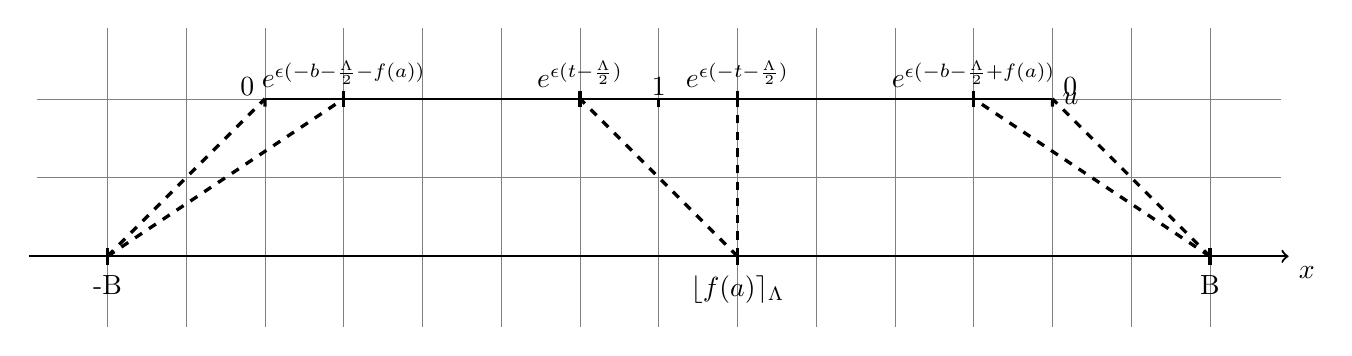
\begin{tikzpicture}
%%%%%%%%%%%%%%%%%%Draw Backgraound Grids%%%%%%%%%%%%%%%
\draw[step=1cm,gray,very thin] (-0.9,-0.9) grid (14.9,2.9);

%%%%%%%%%%%%%%Draw Uniform variable u Line%%%%%%%%%%%%%%
\draw[thick] (2,2) -- (12, 2) node[anchor= west] {$u$};
%%%%%%%%%%%%%%%%%%%Draw The Output Line%%%%%%%%%%%%%%%%%%
\draw[thick,->] (-1,0) -- (15,0) node[anchor=north west] {$x$};
%%%%%%%%%%%$$$%%%Draw Ticks on The Output Line%%%%%%%%%%%
\draw[very thick] (0 cm,3pt) -- (0 cm,-3pt) node[anchor=north] {-B};
\draw[very thick] (14 cm,3pt) -- (14 cm,-3pt) node[anchor=north] {B};
\draw[very thick] (8, 3pt) -- (8, -3pt) node[anchor=north] {$\round{f(a)}_{\Lambda}$};

%%%%%%%%%%%%%%Draw Ticks on The Uniform Line%%%%%%%%%%%
\draw[very thick] (2 ,2) -- (2 cm,1.9)
node[anchor=south east] {0};
\draw[very thick] (3 ,2.1) -- (3, 1.9);

\draw[very thick] (12 ,2) -- (12 cm, 1.9)
node[anchor=south west] {0};
\draw[very thick] (11 ,2.1) -- (11, 1.9);

\draw[very thick] (6 , 2.1) -- (6, 1.9);
\draw[very thick] (7 , 2) -- (7, 1.9)
node[anchor=south] {1};
\draw[very thick] (8 , 2.1) -- (8, 1.9);

%%%%%%%%%%%%%%Draw Maps From Uniform to Output%%%%%%%%%%
\draw[very thick, dashed] (0, 0) -- (3, 2)
node[anchor=south]
{$e^{\epsilon(-b - \frac{\Lambda}{2} - f(a))}$};
\draw[very thick, dashed] (0, 0) -- (2, 2) ;

\draw[very thick, dashed] (8, 0) -- (6, 2) node[anchor=south]{$e^{\epsilon(t - \frac{\Lambda}{2})}$};
\draw[very thick, dashed] (8, 0) -- (8, 2) node[anchor=south]{$e^{\epsilon(-t - \frac{\Lambda}{2})}$};

\draw[very thick, dashed] (14, 0) -- (11, 2) node[anchor=south]{$e^{\epsilon(-b - \frac{\Lambda}{2} + f(a))}$};
\draw[very thick, dashed] (14, 0) -- (12, 2);

\end{tikzpicture}
\\
%
where $b$ is the greatest rounding of $\Lambda$ that is smaller than $B$ and $t = \round{f(a)}_{\Lambda} - f(a)$.


Given the $f(a) = \round{f(a)}_{\Lambda} = 0$, we have following maps from the output of $\snap$ mechanism to uniformly distributed $u \in (0, 1]$.\\
%
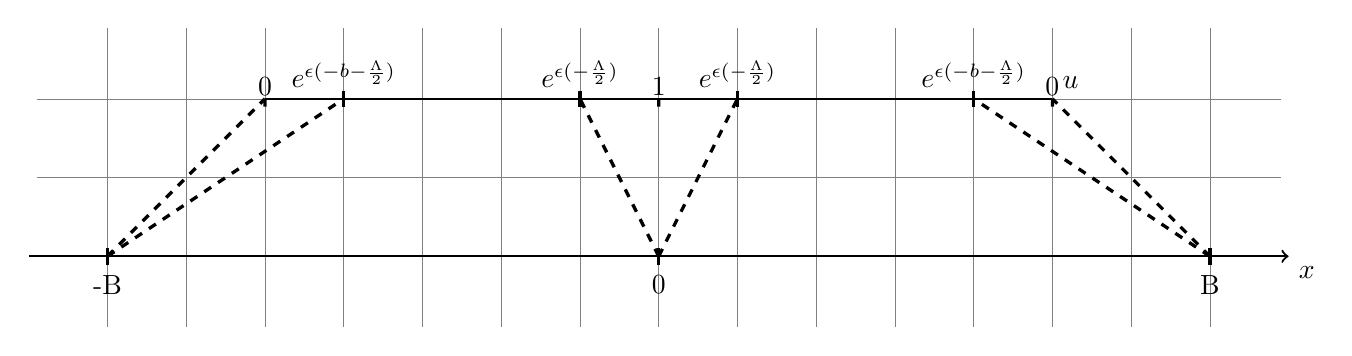
\begin{tikzpicture}
%%%%%%%%%%%%%%%%%%Draw Backgraound Grids%%%%%%%%%%%%%%%
\draw[step=1cm,gray,very thin] (-0.9,-0.9) grid (14.9,2.9);

%%%%%%%%%%%%%%Draw Uniform variable u Line%%%%%%%%%%%%%%
\draw[thick] (2,2) -- (12, 2) node[anchor=south west] {$u$};
%%%%%%%%%%%%%%%%%%%Draw The Output Line%%%%%%%%%%%%%%%%%%
\draw[thick,->] (-1,0) -- (15,0) node[anchor=north west] {$x$};
%%%%%%%%%%%$$$%%%Draw Ticks on The Output Line%%%%%%%%%%%
\draw[very thick] (0 cm,3pt) -- (0 cm,-3pt) node[anchor=north] {-B};
\draw[very thick] (14 cm,3pt) -- (14 cm,-3pt) node[anchor=north] {B};
\draw[very thick] (7 cm,3pt) -- (7 cm,-3pt) node[anchor=north] {0};
%%%%%%%%%%%%%%Draw Ticks on The Uniform Line%%%%%%%%%%%
\draw[very thick] (2 ,2) -- (2 cm,1.9) node[anchor=south] {0};
\draw[very thick] (12 ,2) -- (12 cm, 1.9) node[anchor=south] {0};
\draw[very thick] (7 , 2) -- (7 cm,1.9) node[anchor=south] {1};
\draw[very thick] (3 ,2.1) -- (3, 1.9);

\draw[very thick] (6 , 2.1) -- (6, 1.9);

\draw[very thick] (8 , 2.1) -- (8, 1.9);
\draw[very thick] (11 ,2.1) -- (11, 1.9);

%%%%%%%%%%%%%%Draw Maps From Uniform to Output%%%%%%%%%%
\draw[very thick, dashed] (0, 0) -- (3, 2) node[anchor=south]{$e^{\epsilon(-b - \frac{\Lambda}{2})}$};
\draw[very thick, dashed] (0, 0) -- (2, 2) ;

\draw[very thick, dashed] (7, 0) -- (6, 2) node[anchor=south]{$e^{\epsilon(- \frac{\Lambda}{2})}$};
\draw[very thick, dashed] (7, 0) -- (8, 2) node[anchor=south]{$e^{\epsilon(- \frac{\Lambda}{2})}$};

\draw[very thick, dashed] (14, 0) -- (11, 2) node[anchor=south]{$e^{\epsilon(-b - \frac{\Lambda}{2})}$};
\draw[very thick, dashed] (14, 0) -- (12, 2);

\end{tikzpicture}

Assuming that $f(a) \in [-B, B]$, otherwise we can always redefine the $f(a)$ restricting its output in this range.
The probability of obtaining output $x$ from $\snap$ mechanism can be calculated by cases of $x$:
\begin{itemize}
	\item[\textbf{case}] $x = -B$

	In this case, we know $s = 1$.\\
	We have: $\round{f(a) + \frac{1}{\epsilon} \ln(u)}_{\Lambda} \leq -B $.\\
	%
	Since $b$ is the greatest rounding of $\Lambda$ that is smaller than $B$,
	then $-b$ is the smallest rounding of $\Lambda$ that is greater than $-B$, we have:
	$f(a) + \frac{1}{\epsilon} \ln(u) < -b - \frac{\Lambda}{2}$.\\
	%
	Then we get:
	{\color{red}
	$u \in 
	\big(
	0, e^{\epsilon (-b - \frac{\Lambda}{2} - f(a))}
	\big)$
	}

	\item[\textbf{case}] $x \in (-B, \round{f(a)}_{\Lambda})$
	
	In this case, we know $s = 1$ 
	and $x \in \big[-b, \round{f(a)}_{\Lambda} - \Lambda\big]$.\\
	%
	We have: $\round{f(a) + \frac{1}{\epsilon} \ln(u)}_{\Lambda} = x $.\\
	%
	By the rule of rounding, we get:
	{\color{red}
	$u \in 
	\bigg[
	e^{\epsilon (x - \frac{\Lambda}{2} - f(a))},
	e^{\epsilon (x + \frac{\Lambda}{2} - f(a))}
	\bigg)$}.\\
	%
	By the range of x, we get:
	{\color{red}
	$u \in 
	\bigg[
	e^{\epsilon (-b - \frac{\Lambda}{2} - f(a))},
	e^{\epsilon (t - \frac{\Lambda}{2})}
	\bigg)$}.


	\item[\textbf{case}] $x = \round{f(a)}_{\Lambda}$

	\begin{itemize}
		\item[\textbf{subcase}] $s = 1$\\
		%
		In this case, we have: $\round{f(a) + \frac{1}{\epsilon} \ln(u)}_{\Lambda} = \round{f(a)}_{\Lambda}$.\\
		%
		Then we can get:
		$u \in 
		\big[
		e^{\epsilon(t - \frac{\Lambda}{2})},
		e^{\epsilon(t + \frac{\Lambda}{2})}
		\big]$.\\
		%
		Since $t = \round{f(a)}_{\Lambda} - f(a)$, we know: $- \frac{\Lambda}{2} \leq t \leq \frac{\Lambda}{2}$. So we can get: $e^{\epsilon(t + \frac{\Lambda}{2})} > 1$.\\
		%
		Since $u \in (0, 1]$, we have:
		{\color{red}
		$u \in 
		\big[
		e^{\epsilon(t - \frac{\Lambda}{2})}, 1
		\big]$
		}.

		\item[\textbf{subcase}] $s = -1$\\
		%
		By the symmetric of the range, we can get:
		{\color{red}
		$u \in 
		\big[
		e^{\epsilon(- t - \frac{\Lambda}{2})}, 1
		\big]$
		}.

	\end{itemize}
	
	\item[\textbf{case}] $x \in (\round{f(a)}_{\Lambda}, B)$
	
	In this case, we know $s = -1$ 
	and $x \in \big[
	\round{f(a)}_{\Lambda} + \Lambda, b \big]$.\\
	%
	We have: $\round{f(a) - \frac{1}{\epsilon} \ln(u)}_{\Lambda} = x $.\\
	%
	By the rule of rounding, we get:
	{\color{red}
	$u \in 
	\bigg(
	e^{\epsilon (f(a) - \frac{\Lambda}{2} - x)},
	e^{\epsilon (f(a) + \frac{\Lambda}{2} - x)}
	\bigg]$}.\\
	%
	By the range of x, we get:
	{\color{red}
	$u \in 
	\bigg(
	e^{\epsilon (-b - \frac{\Lambda}{2} + f(a))},
	e^{\epsilon (-t - \frac{\Lambda}{2})}
	\bigg]$}.
	

	\item[\textbf{case}] $x = B$

	In this case, we know $s = -1$.\\
	%
	We have: $\round{f(a) - \frac{1}{\epsilon} \ln(u)}_{\Lambda} \geq B $.\\
	%
	Since $b$ is the greatest rounding of $\Lambda$ that is smaller than $B$, we have:
	$f(a) - \frac{1}{\epsilon} \ln(u) \geq b + \frac{\Lambda}{2}$.\\
	%
	Then we get:
	{\color{red}
	$u \in 
	\big(
	0, e^{\epsilon (-b - \frac{\Lambda}{2} + f(a))}
	\big)$
	}
\end{itemize}

\begin{thm}
$\snap$ mechanism is $\epsilon$-differentially private.
\end{thm}

\begin{proof}[$\epsilon$-differential privacy of $\snap$ mehcnaism]
Given two adjacent database $a$ and $a'$, where $f(a) = \round{f(a)}_{\Lambda} = 0$ and $f(a') = \round{f(a')}_{\Lambda} = 1$, the proof is developed by cases of the output of $x = \snap(a)$, $y = \snap(a')$.

\begin{itemize}
	\item[\textbf{case}] $-B$
	\[
	\frac{Pr[x = -B]}{Pr[y = -B]} 
	= \frac{\frac{1}{2}(
				e^{(-b -\frac{\Lambda}{2})\epsilon})}
				{\frac{1}{2}(
				e^{(-b -\frac{\Lambda}{2} - 1)\epsilon})} \\
	= e^{\epsilon}
	\]


	\item[\textbf{case}] $(-B, 0)$
	\[
	\frac{Pr[x \in (-B, 0)]}{Pr[y \in (-B, 0)]} 
	= \frac{\frac{1}{2}(
				e^{-\frac{\Lambda}{2}\epsilon}
				- e^{(-b -\frac{\Lambda}{2})\epsilon})}
				{\frac{1}{2}(
				e^{(-\frac{\Lambda}{2} - 1)\epsilon}
				- e^{(-b -\frac{\Lambda}{2} - 1)\epsilon})} \\
	= e^{\epsilon}
	\]

	{\color{red}
	\item[\textbf{case}] $0$
	\[
	\frac{Pr[x \in (-B, 0)]}{Pr[y \in (-B, 0)]} 
	= \frac{(1 - e^{-\frac{\Lambda}{2}\epsilon})}
			{\frac{1}{2}(
				e^{(\frac{\Lambda}{2} - 1)\epsilon}
				- e^{(-\frac{\Lambda}{2} - 1)\epsilon})}
	=
	\]


	\item[\textbf{case}] $1$
	\[
	\frac{Pr[x \in (-B, 0)]}{Pr[y \in (-B, 0)]} 
	= \frac{\frac{1}{2}(
				e^{(\frac{\Lambda}{2} - 1)\epsilon}
				- e^{(-\frac{\Lambda}{2} - 1)\epsilon})}
			{(1 - e^{-\frac{\Lambda}{2}\epsilon})}
	=
	\]

	}

	\item[\textbf{case}] $(1, B)$
	\[
	\frac{Pr[x \in (1, B)]}{Pr[y \in (1, B)]} 
	= \frac{\frac{1}{2}(
				e^{(-\frac{\Lambda}{2} - 1)\epsilon}
				- e^{(-b -\frac{\Lambda}{2} - 1)\epsilon})}
				{\frac{1}{2}(
				e^{-\frac{\Lambda}{2}\epsilon}
				- e^{(-b -\frac{\Lambda}{2})\epsilon})} \\
	= e^{-\epsilon}
	\]
	\item[\textbf{case}] $B$
	\[
	\frac{Pr[x = B]}{Pr[y = B]} 
	= \frac{\frac{1}{2}(
				e^{(-b -\frac{\Lambda}{2})\epsilon})}
				{\frac{1}{2}(
				e^{(-b -\frac{\Lambda}{2} + 1)\epsilon})} \\
	= e^{-\epsilon}
	\]



\end{itemize}

\end{proof}
\newpage
\bibliographystyle{plain}
\bibliography{verifysnap.bib}



\end{document}















